The effective asymmetries \Acpprime are obtained after implementing the fitting procedure described in Section~\ref{sec:fitresult}.
The final results for \Acpprime in each lepton-flavor channel are displayed in Fig.~\ref{fig:unblind_result} and the values given in Table~\ref{tab:final_result}.
The correlations between the dominant sources of systematic uncertainty are around 0.3 and only affect the measurement of \Acpprime on the order of 0.001\%.
The results from the previous CMS search at \oldTeV~\cite{CPVtop:CMSresult} are shown for comparison in Fig.~\ref{fig:unblind_result}.
There is no statistically significant evidence for CPV from the present analysis in either lepton-flavor channel for any of the CP observables.
The measured \Acpprime values are in agreement with the SM expectations and have uncertainties roughly a factor of 3 smaller than the previous CMS result.

\begin{figure}[!t]
    \centering
    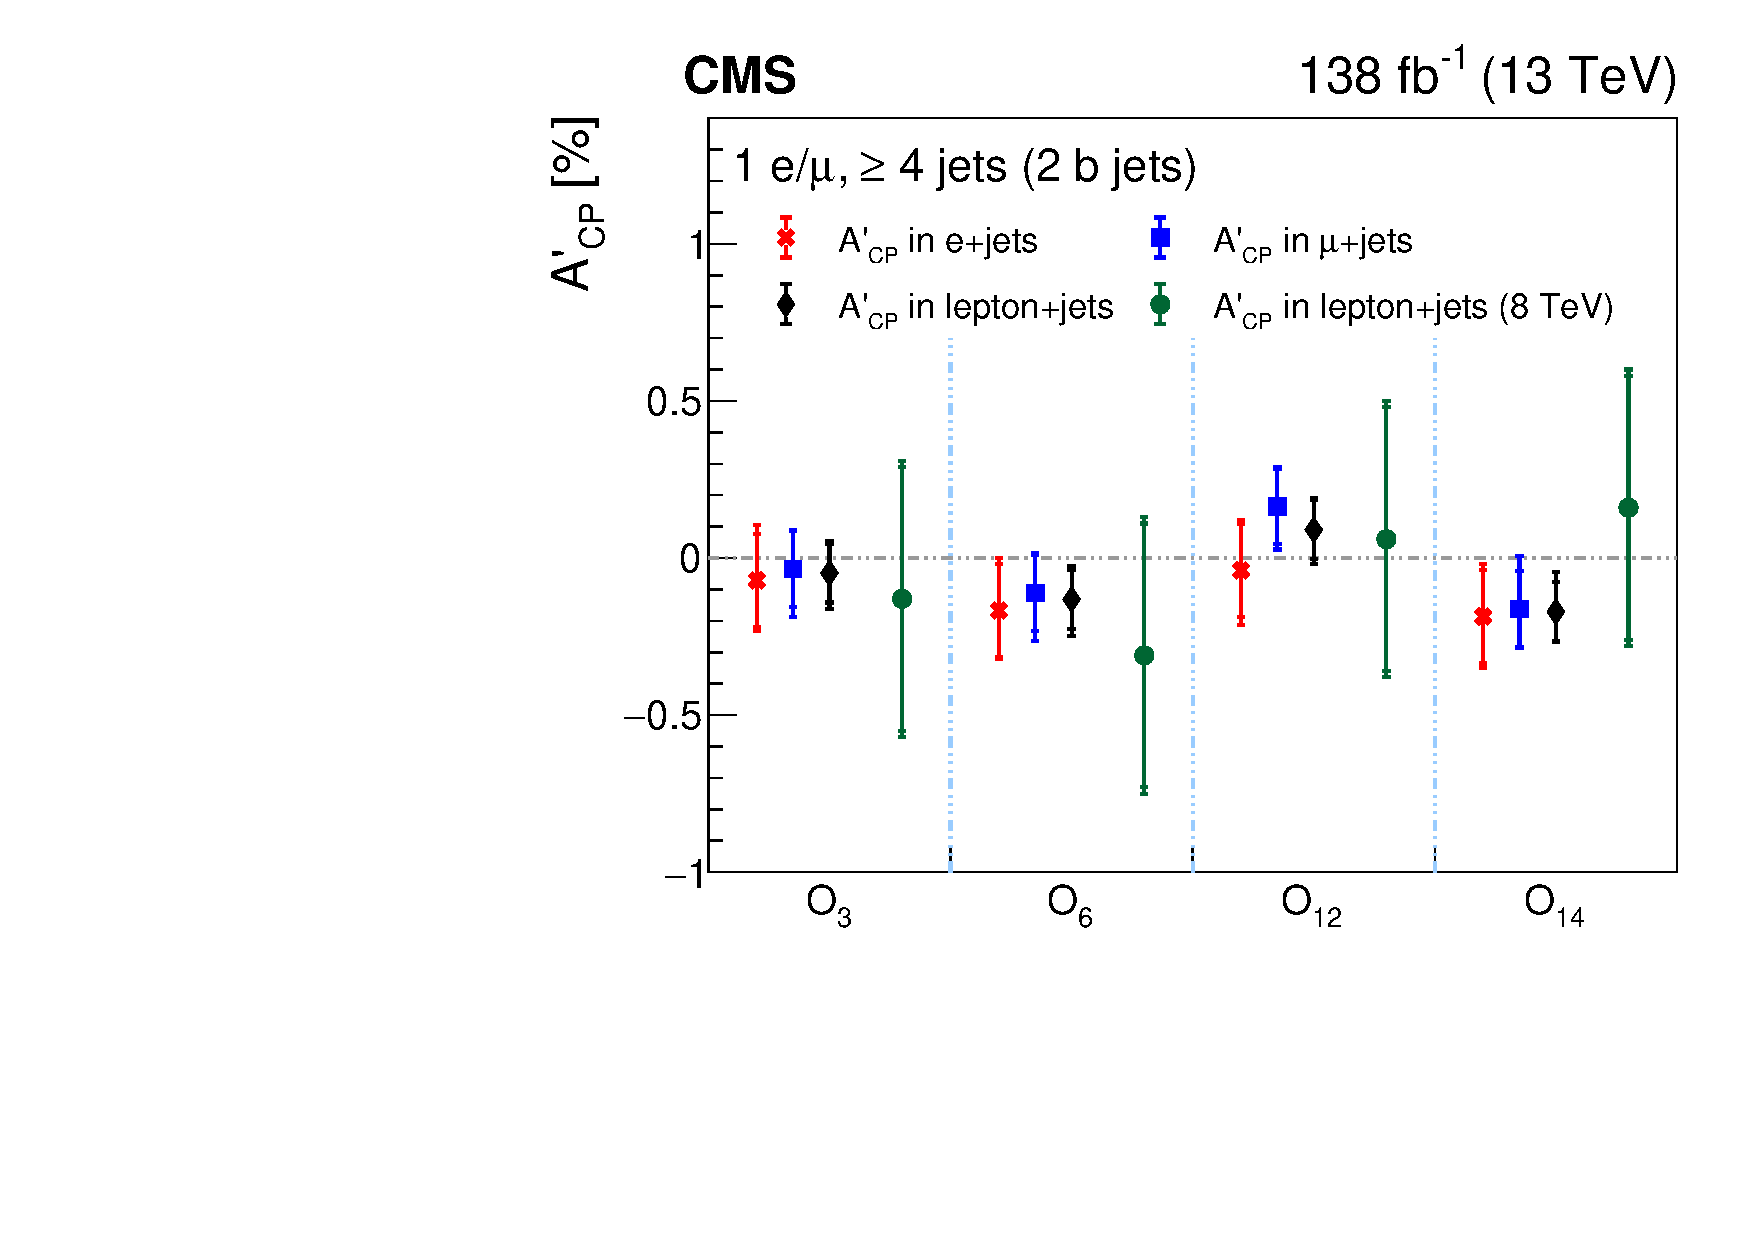
\includegraphics[width=0.7\textwidth]{figure/acp_combined_results.pdf}
    \caption[The measured effective asymmetries \Acpprime for each CP observable.]
    {
        The measured effective asymmetries \Acpprime for each CP observable from the electron, muon, and combined lepton+jets channels.
        The results from the previous CMS measurement at \oldTeV~\cite{CPVtop:CMSresult} are shown by the green circles.
        The inner vertical bars on the symbols represent the statistical uncertainty, and the outer bars the statistical and systematic uncertainties added in quadrature.
    }
    \label{fig:unblind_result}
\end{figure}

\begin{table}[!t]
    \caption[The measured effective asymmetries \Acpprime in percent for each of the CP observables.]
    {
        The measured effective asymmetries \Acpprime in percent for each of the CP observables for the electron, muon, and combined data samples.
        The first uncertainty is statistical and the second is systematic.
        The statistical uncertainties are the same for each lepton type because the numbers of signal events are the same.
    }
    \label{tab:final_result}
    \centering\renewcommand\arraystretch{1.4}
    \begin{tabular}{cccc}
        \multicolumn{4}{c}{\Acpprime (\%)}\\
        & \ejets & \mjets & Combined\\
        \hline
        \Othree
        & $-0.07 \pm 0.15\,^{+0.09}_{-0.06}$
        & $-0.04 \pm 0.12\,^{+0.02}_{-0.09}$
        & $-0.05 \pm 0.09\,^{+0.04}_{-0.07}$\\
        \Osix
        & $-0.17 \pm 0.15\,^{+0.08}_{-0.04}$
        & $-0.11 \pm 0.12\,^{+0.04}_{-0.09}$
        & $-0.13 \pm 0.09\,^{+0.05}_{-0.07}$\\
        \Otwelve
        & $-0.04 \pm 0.15\,^{+0.06}_{-0.09}$
        & $+0.16 \pm 0.12\,^{+0.04}_{-0.07}$
        & $+0.09 \pm 0.09\,^{+0.03}_{-0.05}$\\
        \Ofourteen
        & $-0.19 \pm 0.15\,^{+0.08}_{-0.07}$
        & $-0.16 \pm 0.12\,^{+0.12}_{-0.03}$
        & $-0.17 \pm 0.09\,^{+0.09}_{-0.02}$\\
    \end{tabular}
\end{table}
